%
%
%   LQuiz 14 : 2022--03--29 (T)
%
%

\section{Exercise}

% Reference : SHW
% Graphing tool : https://www.desmos.com/calculator

(4 pt) Let $f : \reals \rightarrow \reals$ be the function whose rule of assignment is
\begin{align*}
f(x)
=
\begin{dcases*}
2 x - x^{2}					&	if $x \leq 2$		\\
\sin\left(\frac{\pi}{2} x\right)	&	if $x \geq 2$
\end{dcases*}
\end{align*}
The function $f$ is graphed below. This exercise explores the signed area under the graph of $f$ from $x = 0$ to $x = 4$.



\begin{enumerate}[label=(\alph*)]
\item\label{itm : LQ14a} (1 pt) Briefly (!) explain why we can't use finite geometry to find the exact value of $\int_{0}^{4} f(x) \spaceIntd \intd x$.
\end{enumerate}

\spaceSolution{0.5in}{% Begin solution.
We cannot use finite geometry to compute the exact signed area between the graph of $f(x)$ and the $x$-axis, because we cannot partition the graph of $f(x)$ into ``nice'' geometric shapes for which we know exact area formulas.}% End solution.



\begin{enumerate}[resume,label=(\alph*)]
\item\label{itm : LQ14b} (1 pt) On separate graphs below, draw a lower sum and an upper sum, each with four intervals of width $1$. Use these to compute a lower and upper estimate for $\int_{0}^{4} f(x) \spaceIntd \intd x$.
\begin{center}
%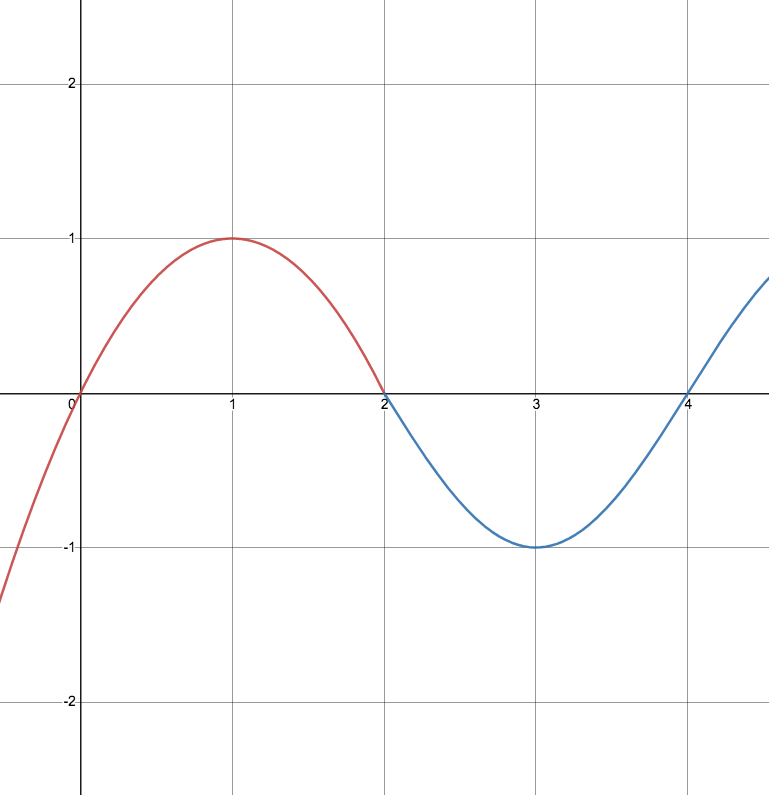
\includegraphics[scale=0.18]{\filePathGraphics/LQ14_Graph.png}% Activate for quiz.
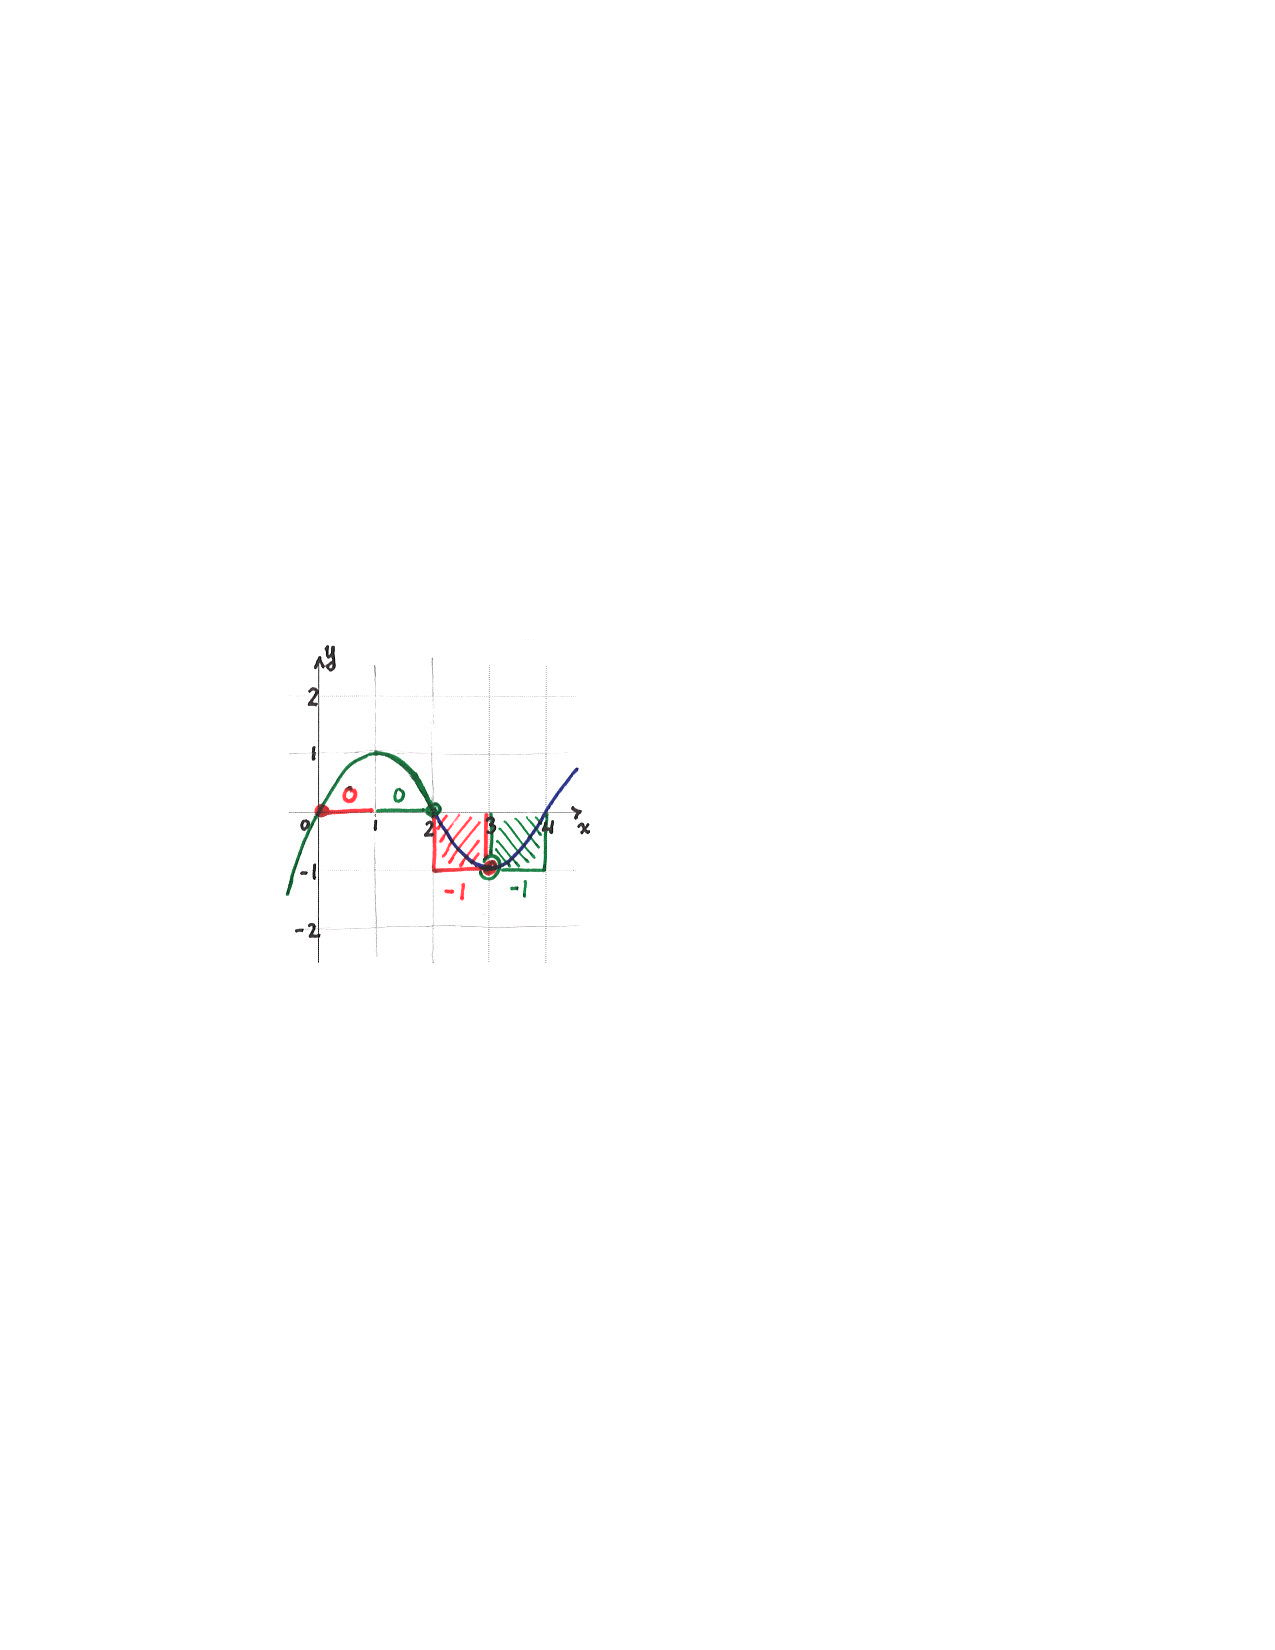
\includegraphics[scale=0.8]{\filePathGraphics/LQ14_Graph_Lower.pdf}% Activate for solutions.
\hspace{1in}
%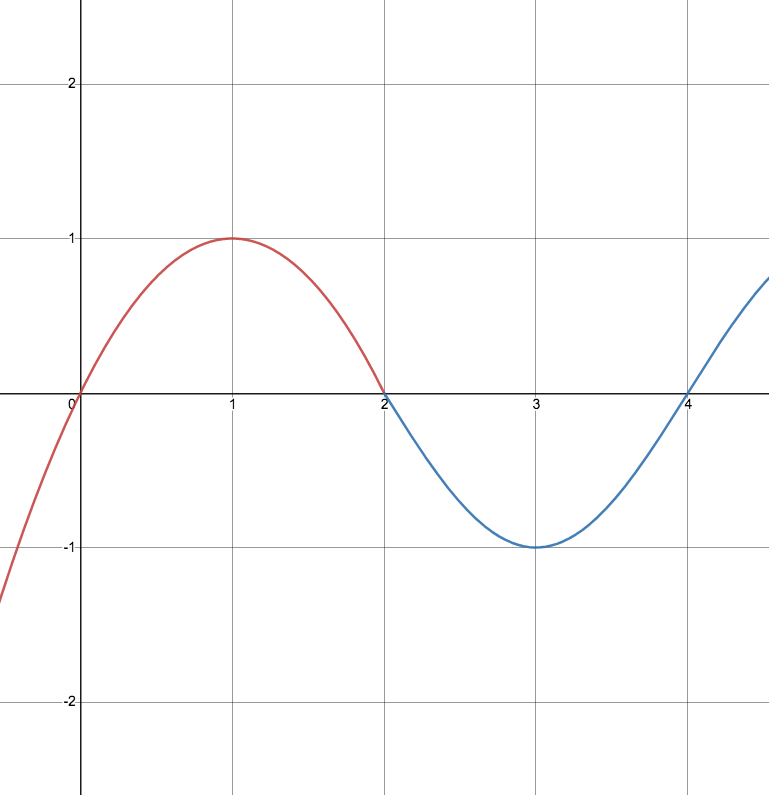
\includegraphics[scale=0.18]{\filePathGraphics/LQ14_Graph.png}% Activate for quiz.
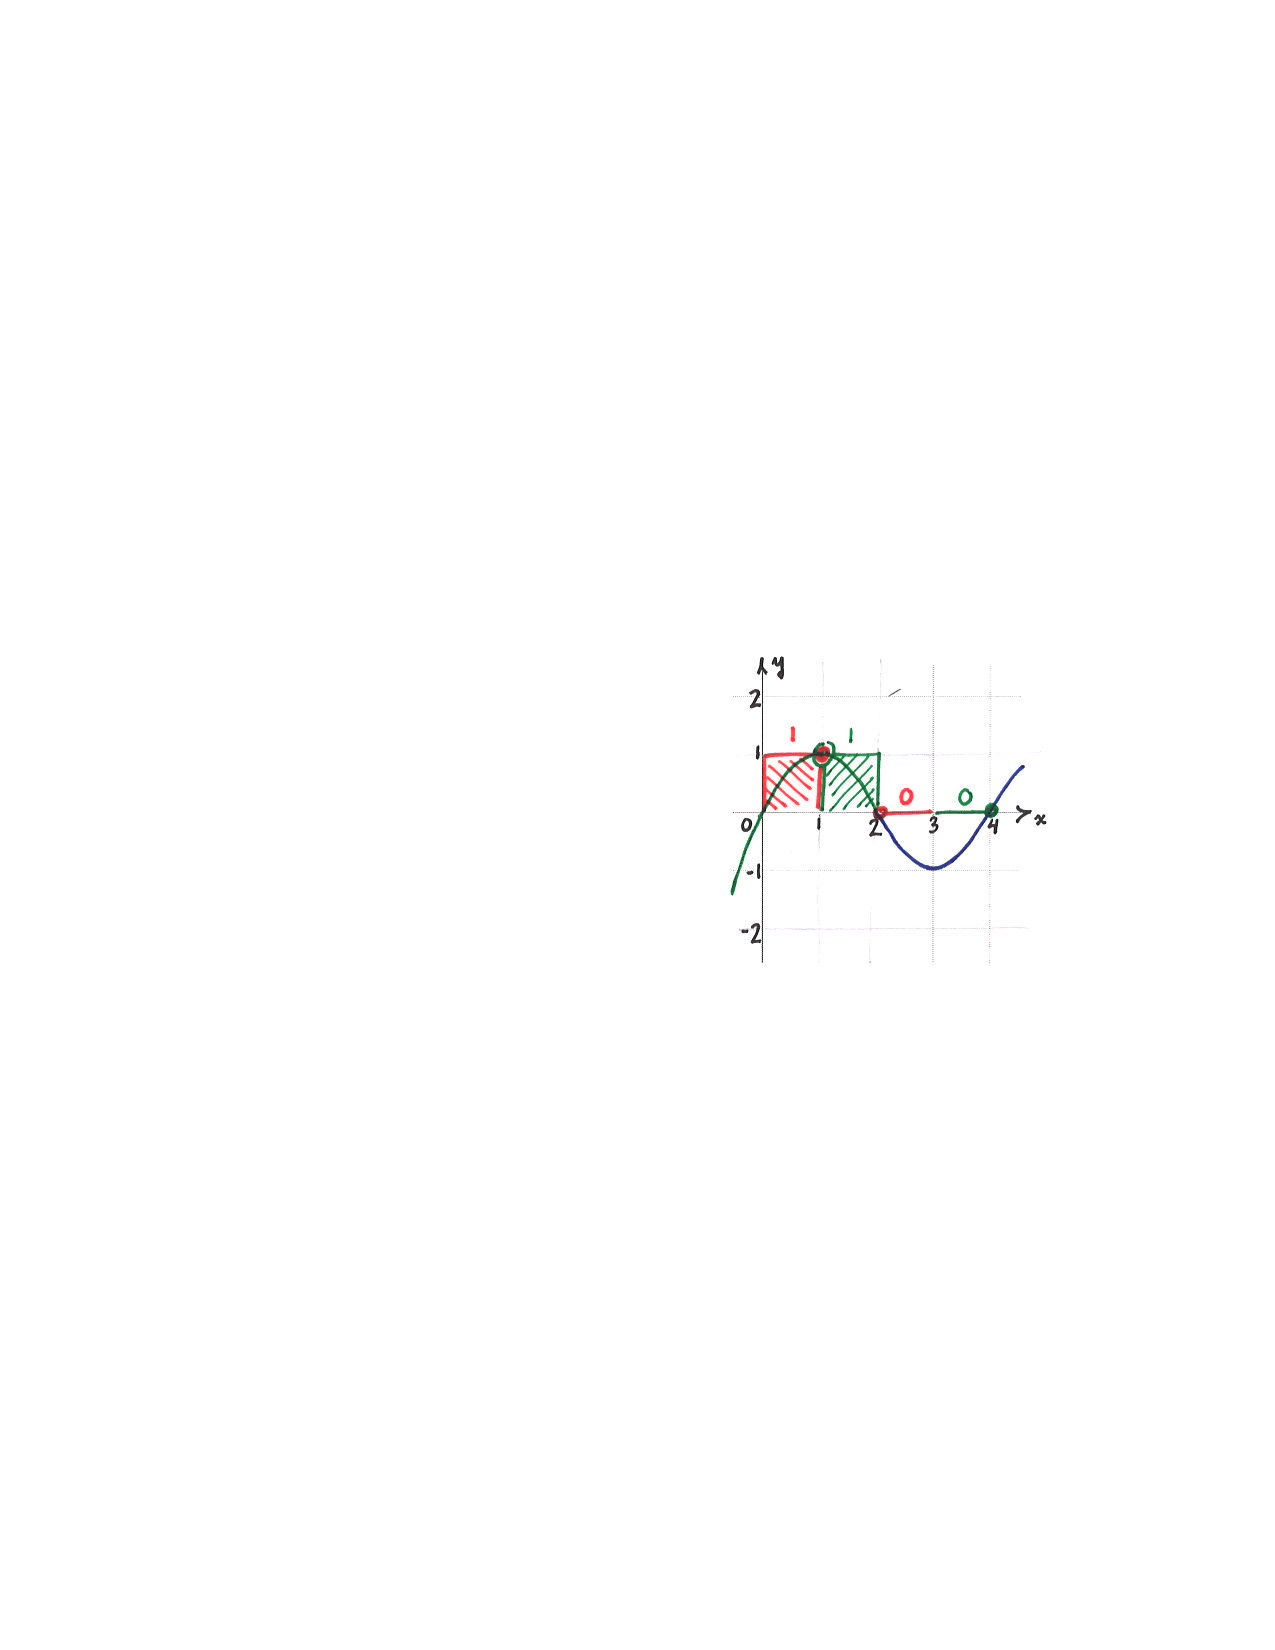
\includegraphics[scale=0.8]{\filePathGraphics/LQ14_Graph_Upper.pdf}% Activate for solutions.
\\
Lower sum ($L$)
\hspace{2in}
Upper sum ($U$)
\end{center}
\end{enumerate}

\spaceSolution{0.25in}{% Begin solution.
The lower and upper sums are sketched above. We compute
\begin{align*}
L
&=
1 (0) + 1 (0) + 1 (-1) + 1 (-1)
=
-2
&
U
&=
1 (1) + 1 (1) + 1 (0) + 1 (0)
=
2
\end{align*}}% End solution.



\begin{enumerate}[resume,label=(\alph*)]
\item\label{itm : LQ14c} (2 pt) Find an antiderivative $F_{i}(x)$ for each ``piece'' of $f(x)$. Use these antiderivatives and the fundamental theorem of calculus to compute the integrals on the right side of
\begin{align}
\int_{0}^{4} f(x) \spaceIntd \intd x
=
\int_{0}^{2} f(x) \spaceIntd \intd x
+
\int_{2}^{4} f(x) \spaceIntd \intd x%
\label{eq : LQ14 Piecewise Integral}
\end{align}
Add your results to determine the integral on the left side. Show that $L \leq \int_{0}^{4} f(x) \spaceIntd \intd x \leq U$..
\end{enumerate}

\spaceSolution{1in}{% Begin solution.
By ``running the derivative in reverse'', and tweaking our original guess as needed, we find the antiderivatives
\begin{align*}
F_{1}(x)
&=
x^{2} - \frac{1}{3} x^{3}
&
F_{2}(x)
&=
-\frac{2}{\pi} \cos\left(\frac{\pi}{2} x\right)
\end{align*}
Note that (i) these are not (!) the most general antiderivatives of the corresponding $f_{i}(x)$---they are particular antiderivatives of $f_{i}(x)$, where we have chosen the constant $C_{i} = 0$ in both cases; and (ii) we can quickly check that each $F_{i}(x)$ is indeed an antiderivative of the corresponding $f_{i}(x)$, by computing the derivative of the former:
\begin{align*}
F_{1}'(x)
&=
2 x - \frac{1}{3} 3 x^{2}
=
2 x - x^{2}
=
f_{1}(x)
\\
F_{2}'(x)
&=
-\frac{2}{\pi} \left[-\frac{\pi}{2} \sin\left(\frac{\pi}{2} x\right)\right]
=
\sin\left(\frac{\pi}{2} x\right)
=
f_{2}(x)
\end{align*}

We may use these antiderivatives in the fundamental theorem of calculus to compute the integrals on the right side of Equation \eqref{eq : LQ14 Piecewise Integral}:
\begin{align*}
\int_{0}^{2} f(x) \spaceIntd \intd x
&=
F_{1}(2) - F_{1}(0)
\\
&=
\left[(2)^{2} - \frac{1}{3} (2)^{3}\right] - \left[(0)^{2} - \frac{1}{3} (0)^{3}\right]
\\
&=
\left[4 - \frac{8}{3}\right] - [0 - 0]
\\
&=
\frac{4}{3}
\\
\int_{2}^{4} f(x) \spaceIntd \intd x
&=
F_{2}(4) - F_{2}(2)
\\
&=
\left[-\frac{2}{\pi} \cos\left(\frac{\pi}{2} (4)\right)\right] - \left[-\frac{2}{\pi} \cos\left(\frac{\pi}{2} (2)\right)\right]
\\
&=
\left[-\frac{2}{\pi} (1)\right] - \left[-\frac{2}{\pi} (-1)\right]
\\
&=
-\frac{4}{\pi}
\end{align*}
Therefore
\begin{align*}
\int_{0}^{4} f(x) \spaceIntd \intd x
&=
\int_{0}^{2} f(x) \spaceIntd \intd x
+
\int_{2}^{4} f(x) \spaceIntd \intd x
\\
&=
\frac{4}{3} - \frac{4}{\pi}
\approx
0.0601
\end{align*}
We note that
\begin{align*}
L
&=
-2
&
&\leq
&
\int_{0}^{4} f(x) \spaceIntd \intd x
&\approx
0.0601
&
&\leq
&
U
&=
2
\end{align*}
as required by the theory of lower and upper sums.

Remarks.
\begin{enumerate}
\item The total signed area is close to zero, as suggested by the graph of $f$.
\item Even without a calculator, we can know for sure that $\frac{4}{3} - \frac{4}{\pi}$ is positive, by the following argument (the symbol ``$\Leftrightarrow$'' means ``if and only if'' or ``is equivalent to''):
\begin{align*}
3
&<
\pi
\approx
3.1416
&
&\Leftrightarrow
&
\frac{1}{3}
&>
\frac{1}{\pi}
&
&\Leftrightarrow
&
\frac{4}{3}
&>
\frac{4}{\pi}
&
&\Leftrightarrow
&
\frac{4}{3} - \frac{4}{\pi}
&>
0
\end{align*}
\end{enumerate}}% End solution.